\documentclass[a4paper,11pt]{article}
\usepackage[english]{babel}
\usepackage[utf8]{inputenc}
\usepackage{amsmath}
\usepackage{threeparttable}
\usepackage{amsthm}
\usepackage{amsfonts}
\usepackage{amssymb}
\usepackage{graphicx}
\usepackage[boxed]{algorithm}
\usepackage{algorithmic}
\usepackage[natbib=true]{biblatex}
%\usepackage{fancyhdr}
%\usepackage{natbib}
%\usepackage[natbib=true]{biblatex}
%\usepackage{epstopdf}
%\usepackage{float}
%\usepackage{url}
\usepackage[pdftex]{hyperref}
\usepackage{enumerate}
\usepackage{array,ragged2e}
\usepackage{listings}
\lstset{language=C}

\newcommand{\R}{\mathbb{R}}
\newcommand{\N}{\mathbb{N}}
\newcommand{\Z}{\mathbb{Z}}
\newcommand{\C}{\mathbb{C}}
\newcommand{\dx}{\, \mathrm{d}}
\newcommand{\de}{\partial}

\newcolumntype{C}[1]{>{\Centering}m{#1}}

\newtheorem{thm}{Theorem}[section]
\renewcommand{\qedsymbol}{$\lozenge$}

%\bibliographystyle{unsrt}

%\hoffset = 0cm
%\voffset = -2cm
%\textheight = 700pt
%\marginparwidth = 0pt
%\textwidth = 450pt
%\oddsidemargin = 0pt
%\evensidemargin = 0pt
%\topmargin = 0pt

\renewcommand{\algorithmicrequire}{\textbf{Input:}}
\renewcommand{\algorithmicensure}{\textbf{Output:}}

\setlength\parindent{0pt}
\setlength{\parskip}{5pt} %%distanza fra i paragrafi

\bibliography{biblio_sieve}

\begin{document}

\title{Parallel Algorithms: The Sieve of Eratosthenes}
\author{Kleopatra Pirpinia}

\date{}

\maketitle

\begin{abstract}
In this report we will discuss a parallel implementation of the sieve of Eratosthenes within the framework of the BSP model, we will estimate its BSP cost and present the results of various numerical experiments.We will also add some minor modifications in order to check the Goldbach conjecture as well as to generate pairs of twin prime numbers.
\end{abstract}

\tableofcontents

\pagebreak

\section{Sieve of Eratosthenes}

In mathematics, the sieve of Eratosthenes is a simple, ancient algorithm for finding all prime numbers up to any given number $n$. It does so by iteratively marking as composite (i.e. not prime) the multiples of each prime, starting with the multiples of 2.



\subsection{The sequential algorithm}
The sequential algorithm is the following:


\begin{algorithm}
\begin{algorithmic}
\REQUIRE $n \in \N$
\ENSURE A list with all the primes up to $n$.
\STATE
\IF{$n$ is odd}
\STATE Create the list of numbers $l=[2,3,5,7,\dots,n]$.
\ELSE
\STATE Create the list of numbers $l=[2,3,5,7,\dots,n-1]$.
\ENDIF
\FOR{$p=3,\dots,\sqrt{n}$}
\STATE Remove all the multiples of $p$ from $l$
\STATE $p$ is the next element of $l$
\ENDFOR
\RETURN $l$
\end{algorithmic}
\end{algorithm}

Firstly, note that we will consider only the odd numbers (and 2 of course, which is a prime) up to $n$, which reduces the number of operations we have to perform. 

Furthermore, let us notice that it is sufficient to start crossing out the multiples of $p$ at $p^2$,since all the smaller multiples will have already been crossed out by that time. Therefore, when $p^2$ becomes larger than $n$, the algorithm must stop. In other words, it suffices that $p$ goes only up to $\sqrt{n}$.

\subsubsection{The implementation}


We implement the above algorithm creating firstly the array $l$ of length $\frac{n}{2}$. 

In order to do this, we need to find a convenient correspondence between the elements of the array and their indices. 

In our case it is straightforward that a nice correspondence is $l[i]=2i+1$, with $i \geq 1$. The first element of the array (in the position 0) is set to be always 2.

Furthermore, we want to start crossing out the multiples of every element, and we do this by considering $l[i]$ and doing a cycle with step $2i+1$. 

For example, for $l[1]=3$, we start crossing out its multiples at $l[i+2i+1]=l[4]=9$ and so on. Doing this we get straight to the multiples without controlling every number, and we cross them out instantly setting them equal to 0.

It is then easy to go through $l$ and count the number of primes, and create a new list $l'$ without the 0's.

\subsubsection{The cost}

It is given that the probability of an arbitrary integer $x \geq 2$ to be prime is $\frac{1}{\ln x}$. 

We also know that the number of multiples that we cross out for each number is $$\frac{n}{p}$$ 

Combining this with the fact that $$\displaystyle \sum_{p \leq n}\frac{1}{p}$$ goes asymptotically to $\ln \ln n$ we get that the cost of our algorithm is $O(n \ln \ln n)$. It does not matter asymptotically if we omit the even numbers from the initial array.

\subsection{The parallel algorithm}

For the parallel algorithm, the fact that we only need the primes up to $\sqrt{n}$ in order to cross out all the non primes up to $n$ is fundamental. The idea is that if all the processors have the list of primes up to $\sqrt{n}$, then we can distribute the numbers from $\sqrt{n}$ to $n$ and they'll have all the information they need in order to cross out the multiples in parallel.  

\subsubsection{The implementation}
The parallel algorithm is given below:

\begin{algorithm}[H]
\begin{algorithmic}
\REQUIRE $n \in \N$
\ENSURE The total number of primes below $n$
\end{algorithmic}

\begin{enumerate}
\item[(0)] \begin{algorithmic}
\STATE Compute sequentially the primes up to $\sqrt{n}$ and store it in the array \verb|initialPrimes|.
\STATE
\STATE Create the array \verb|local| of size $b:= \left\lceil \dfrac{n-\sqrt{n}}{2p} \right\rceil$ using block distribution, starting from number $\sqrt{n}+2sb$.
\STATE
\FOR{$z \in \texttt{initialPrimes}$}
\STATE $i:=$ first index such that $\verb|local[i]|=kz$ for some $k \in \N$
\WHILE{$i<b$}
\STATE flag \verb|local[i]| as non-prime
\STATE $i=i+z$
\ENDWHILE
\ENDFOR
\STATE
\STATE $count_s:=0$
\FOR{$x \in local$}
\IF{$x$ is not flagged}
\STATE $count_s=count_s+1$
\ENDIF
\ENDFOR
\end{algorithmic}
\item[(1)] \begin{algorithmic}
\FOR{$t:=0,\dots,p-1$}
\STATE Put $count_s$ in $P(t)$
\ENDFOR
\end{algorithmic}
\item[(2)] \begin{algorithmic}
\STATE $finalCount:=0$
\FOR{$t=0,\dots,p-1$}
\STATE $finalCount = finalCount + count_s$.
\ENDFOR
\end{algorithmic}

\end{enumerate}
\end{algorithm}


As mentioned before, we begin the implementation with a sequential part, using a function $seq(n)$ (which uses the algorithm described in the previous Section) that computes the number of primes up to $n$. So, we make all $p$ processors find the primes up to $\sqrt{n}$ and place them in an array which we call \textit{initialPrimes}. 

Then the parallel part starts: the remaining $n - \sqrt{n}$ numbers are distributed among the processors in blocks, thus there are $\frac{n-\sqrt{n}}{2p}$ numbers on every processor, rounded up (remember that we consider only the odd numbers between 2 and $n$, thus the 2 of the denominator). 

The block distribution was chosen over the cyclic since it permits us to locate easily the multiples: if $k$ is a multiple of $z$ then also $k+z$ is; moreover, as we will see later on, it allows us to find nicely the pairs of twin primes - almost all primes that are twins are adjacent to each other!

Now, every processor starts crossing out the multiples of the initially given primes. However this time we choose to not set them equal to zero, but flag them in a different way instead - we just change the sign and set them negative. This way the value of each element is not lost, and it can still be checked if the flagged number is a multiple of another prime, in order to start ``jumping'' from one multiple to the next, thus saving some extra operations.

After that every processor counts the number of non-flagged entries, and broadcasts this number to all the others; finally all of them then compute the final number of primes.

\subsubsection{The BSP cost}

Based on the remarks we made above, we can give an estimation of the BSP cost. For the sequential part we have

$$\lfloor \sqrt{n} \rfloor \ln \ln \lfloor \sqrt{n} \rfloor$$

For the flagging of multiples in parallel we have

$$\frac{n}{p} \ln \ln n + l$$

Then we have a $(p-1)$-relation in the communication superstep, so the cost is 

$$(p-1)g + l$$

Finally we have $p$ additions in order to compute the final sum. Therefore the overall cost is

$$T= \lfloor \sqrt{n} \rfloor \ln \ln \lfloor \sqrt{n} \rfloor +\frac{n}{p} \ln \ln n + (p-1)g + p + 3l$$
\section{Twin primes}
A \textit{twin prime} is a prime number that differs from another prime by two.

\begin{algorithm}[H]
\begin{algorithmic}
\REQUIRE $n \in \N$ and the arrays as they are at the end of the previous algorithm
\ENSURE The number of twin primes below $n$
\end{algorithmic}


\begin{enumerate}
\item[(0)] \begin{algorithmic}
\STATE $nLocalTwins_s :=0$
\STATE 
\IF{$s=0$}
\FOR{$i=0,\dots,size(\texttt{initialPrimes})-1$}
\IF{\texttt{initialPrimes[i+1]}= \texttt{initialPrimes[i]}+2}
\STATE $nLocalTwins_s = nLocalTwins_s+1$.
\ENDIF
\ENDFOR
\IF{$\texttt{local[0]}$ is prime $\quad \wedge \quad \texttt{initialPrimes[-1]}$ is prime}
\STATE $nLocalTwins_s = nLocalTwins_s+1$. 
\ENDIF
\ENDIF
\STATE
\FOR{$i=0,\dots,b-1$}
\IF{$\texttt{local[i]}$ is prime $\quad \wedge \quad \texttt{local[i+1]}$ is prime}
\STATE $nLocalTwins_s = nLocalTwins_s+1$. 
\ENDIF
\ENDFOR
\STATE
\STATE $flag:=0$
\IF{$\texttt{local[b-1]}$ is prime}
\STATE $flag=1$
\ENDIF
\end{algorithmic}
\item[(1)] \begin{algorithmic}
\IF{$s<p-1$}
\STATE Put $flag$ in $P(s+1)$ into the variable $prevFlag$
\ENDIF
\end{algorithmic}
\item[(2)] \begin{algorithmic}
\IF{$prevFlag=1 \quad \wedge \quad \texttt{local[0]}$ is prime}
\STATE $nLocalTwins_s = nLocalTwins_s+1$. 
\ENDIF
\end{algorithmic}

\item[(3)] \begin{algorithmic}
\FOR{$t:=0,\dots,p-1$}
\STATE Put $nLocalTwins_s$ in $P(t)$
\ENDFOR
\end{algorithmic}

\item[(4)] \begin{algorithmic}
\STATE $totalTwins:=0$
\FOR{$t=0,\dots,p-1$}
\STATE $totalTwins = totalTwins + nLocalTwins_s$.
\ENDFOR
\end{algorithmic}

\end{enumerate}
\end{algorithm}


The above is the algorithm used to compute the number of twin primes from $2$ to $n$, after having used the parallel sieve described in the previous section. Therefore we refer to the same arrays as before and these operations are intended to be executed right after the previous ones, still in the SPMD part.


Note that because we are only considering arrays with odd numbers and we are using the block distribution, twin primes are adjacent to each other. The only case in which this is not true is when this pair is split among two different processors.

The algorithm, substantially, works as follows:

Processor 0 initially does the following operations:
\begin{itemize}
\item it looks for twin primes in the array \texttt{initialPrimes} which contains exclusively the primes up to $\sqrt{n}$
\item it checks whether a pair of twin primes was split between \texttt{initialPrimes} and its local list (note that this processor gets the first chunk of all the numbers to sieve).
\end{itemize}

Then, every processor does the following:
\begin{itemize}

\item it looks for twin prims in its local list
\item it checks whether the last element of the local list is prime, if this is the case the flag is set to 1
\item it sends to the next one the information about the last element of the local list
\item it checks whether there was a pair of twin primes split between him and the previous one
\item it broadcasts the number of twin primes found to all the other processors
\item computes the final number of twin primes
\end{itemize}

\section{Goldbach's Conjecture}
Goldbach's conjecture, one of the most famous problems of number theory, states that any given even integer greater than 2 can be expressed as a sum of 2 primes.

The following is the algorithm used to check its validity up to a given number $n$.



\begin{algorithm}[H]
\begin{algorithmic}
\REQUIRE $n \in \N$ and the arrays as they are at the end of the previous algorithm
\ENSURE The number of non-Goldbach primes below $n$
\end{algorithmic}

\begin{enumerate}
\item[(0)] \begin{algorithmic}
\IF{$s=0$}
\STATE $\texttt{localPrimes}_s := (\texttt{initialPrimes},\mbox{ primes in }\texttt{local})$
\ELSE
\STATE $\texttt{localPrimes}_s := \texttt{local} \mbox{ without the non-primes}$
\ENDIF
\end{algorithmic}

\item[(1)] \begin{algorithmic}
\FOR{$t:=0,\dots,p-1$}
\STATE Put $\texttt{localPrimes}_s$ in $P(t)$.
\ENDFOR
\end{algorithmic}

\item[(2)] \begin{algorithmic}
\STATE create the list \texttt{allPrimes} by ordered concatenation of $\texttt{localPrimes}_s$.
\IF{$n$ is even}
\STATE $largestEven := n$
\ELSE
\STATE $largestEven := n-1$
\ENDIF
\STATE
\STATE $r := \left\lceil \dfrac{largestEven-4}{2p} \right\rceil$
\STATE
\STATE Create the array \verb|listEven| of size $r$ using block distribution, starting from number $4+2rs$
\STATE
\FOR{$i=0,\dots,r-1$}
\FOR{$j=0,\dots,finalCount-1$}
\FOR{$k=j,\dots,finalCount-1$}
\IF{\texttt{allPrimes[j]}+\texttt{allPrimes[k]}=\texttt{listEven[i]}}
\STATE flag \texttt{listEven[i]} as satisfied
\STATE exit from the loops on $j$ and $k$ and continue the one on $i$
\ENDIF
\ENDFOR
\ENDFOR
\ENDFOR
\STATE
\STATE $numberNonGoldbach :=$ amount of number of \texttt{listEven} not satisfied
\end{algorithmic}
\end{enumerate}
\end{algorithm}


\textbf{Remark.} 

Ideally, the algorithm should continue with the communication superstep in which each processor lets the other know its value for $numberNonGoldbach$ and then they should compute the total amount, as done similarly for the amount of primes and pairs of twins; however, we cheated a little bit because we already know that the Goldbach Conjecture has been verified until $ 4 \times 10^{18}$ (so we know that for any number that we might test it would return 0) and because the algorithm just given is already quite expensive, we decided to remove the ``unnecessary'' work.

\section{Benchmarking}

Now, we wanted to measure the performance of our computers in terms of the computing rate $r$, synchronization cost $l$ and communication parameter $g$, running the program \texttt{bspbench}.

We performed this benchmark on the Dutch supercomputer Huygens, a clustered SMP with a total of 3456 cores, and on a MacBook Air with 2 Intel i5 cores @1.7 GHz.

\begin{table}[H]
\begin{center}
\begin{tabular}{|C{2.8cm}|r r r r|}
\hline
\textbf{Machine} & Processors & $r$ (Mflop/s) & $g$ & $l$ \\
\hline
Huygens & 1 & 195.693 & 51.7 & 550.6 \\
& 2 & 195.715 & 55.5 & 1945.7 \\
& 4 & 195.321 & 57.8 & 4051.5 \\
& 8 & 195.480 & 57.4 & 7791.0 \\
& 16 & 195.321 & 60.0 & 15552.7 \\
& 32 & 195.210 & 61.2 & 32539.8 \\
& 64 & 195.487 & 63.2 & 100744.5 \\
& 128 & 195.049 & 116.0 & 213201.8 \\
& 256 & 195.487 & & \\
\hline
Macbook Air & 1 &  251.080 & 50.3 & 663.2\\
& 2 & 253.730 & 75.2 & 4409.5\\
& 4 & 285.837 & 232.2 & 15470.0\\
\hline
\end{tabular}
\caption{Value for $r$, $g$ and $l$ with the benchmark.} \label{tab:bench}
\end{center}
\end{table}

\textbf{Remarks.} We notice that $g$ is always almost the same except in the case when we use 128 processors. This can be explained looking at the structure of Huygens: the fact that there are nodes of 32 cores, makes the communication inside it very fast, and even when there in one adjacent to it it is still ok (this is the case of 64 cores) but when we need more of them, the communication can become slower, since they might be not so near.

\subsection*{Results for \texttt{bsp\_put}}
Here we present some  (for sake of brevity) results we obtained after running \texttt{bspbench} on Huygens and on a Macbook Air:

\begin{figure}[H]
\begin{center}
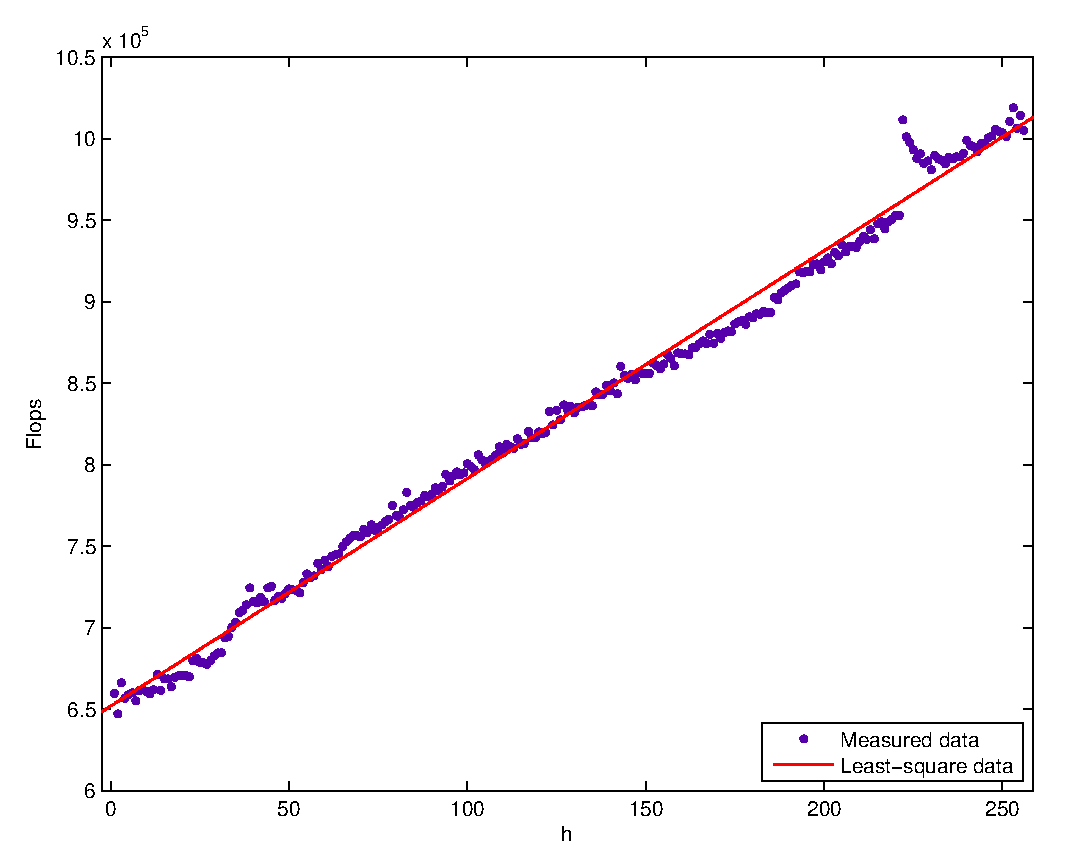
\includegraphics[scale=0.6]{img/32-put}
\end{center}
\caption{Huygens: $p=32$}\label{huy:32}
\end{figure}

\begin{figure}[H]
\begin{center}
\includegraphics[scale=0.6]{img/mb-2-put}
\end{center}
\caption{MacBook Air: $p=2$}\label{mb:2}
\end{figure}



\subsection*{Results for \texttt{bsp\_get} }

We then modified our program to \texttt{bsp\_get} and performed again some measurements:


\begin{figure}[H]
\begin{center}
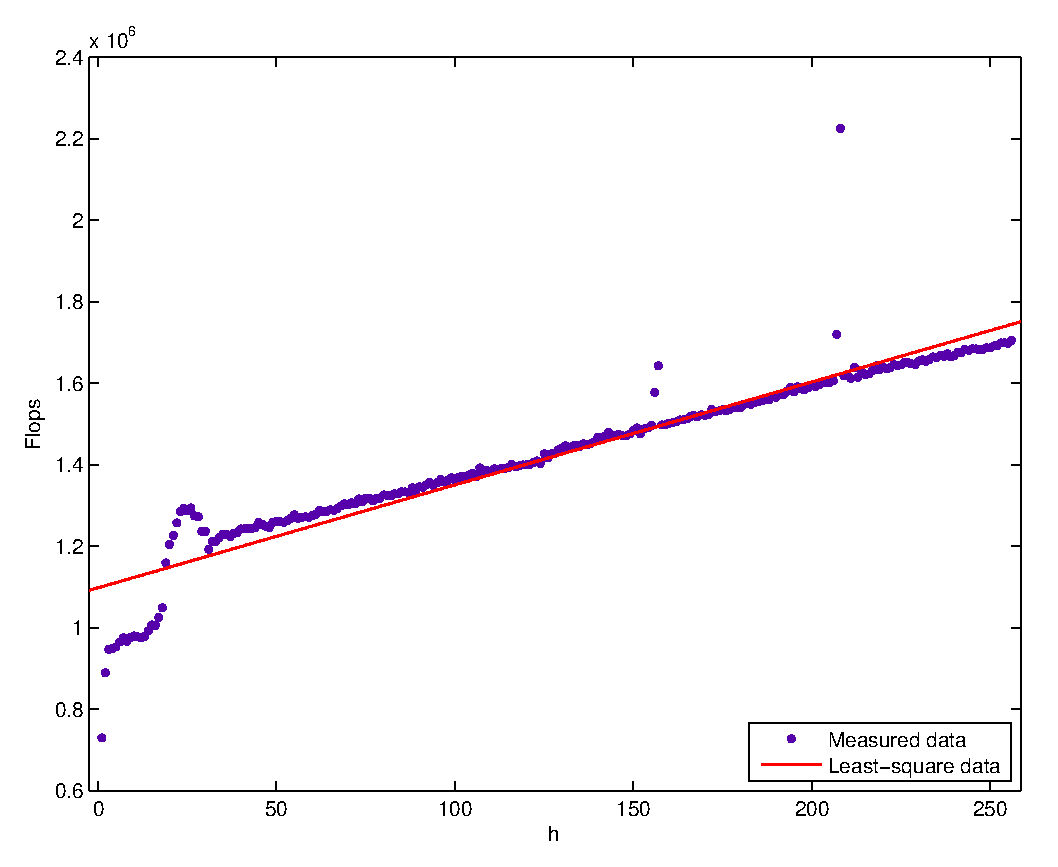
\includegraphics[scale=0.6]{img/32-get}
\end{center}
\caption{Huygens: $p=32$ with \texttt{bsp\_get}}\label{huy:32}
\end{figure}

\begin{figure}[H]
\begin{center}
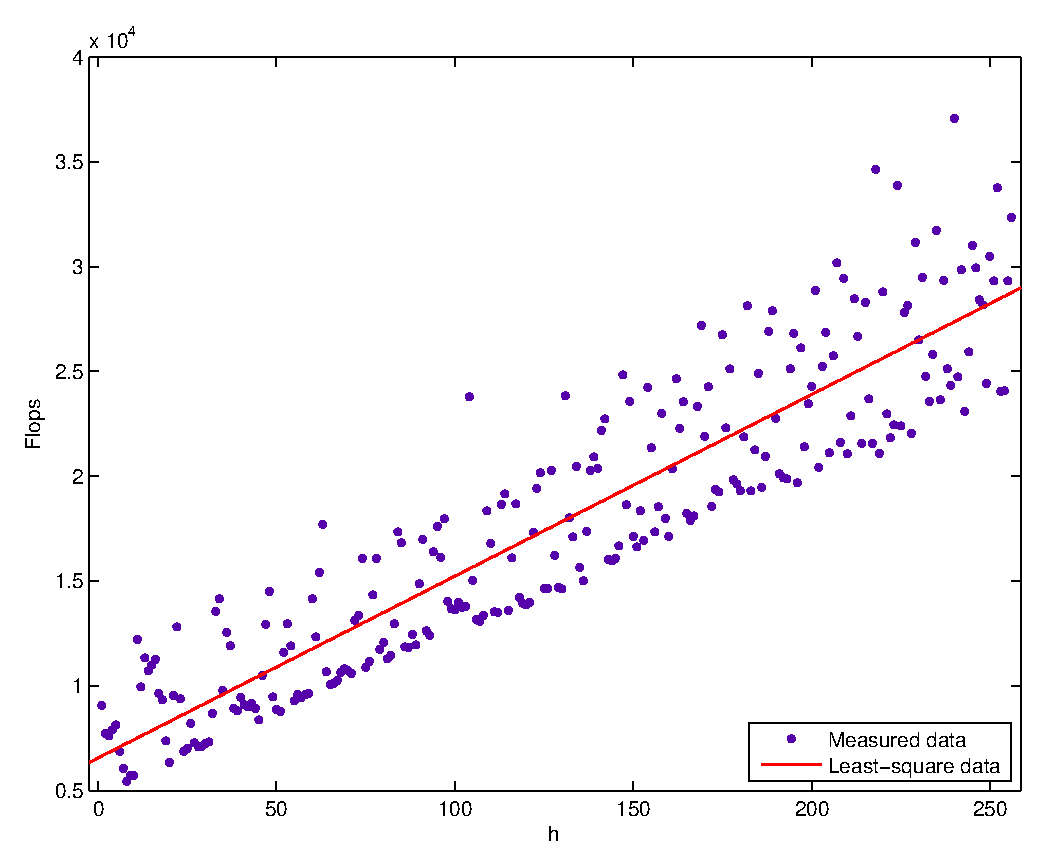
\includegraphics[scale=0.6]{img/mb-2-get}
\end{center}
\caption{MacBook Air: $p=2$ with \texttt{bsp\_get}} \label{mb:2}
\end{figure}

\section{Time measurements}

In order to test the real effectiveness of our program, we decided to test it and compute the prime numbers up to $10^8$ and $10^9$.

\subsection{Huygens}

In the following Tables we give the results obtained from Huygens for $n=10^8$:

\begin{table}[H]
\begin{center}
\begin{tabular}{|r r|}
\hline
p & t (sec) \\
\hline
1 &7.6615\\
2 & 3.4998 \\
4 &1.3157\\
8 &0.6531 \\
16 &0.2228\\
32 &0.1258\\
64 &0.0954\\
128 &0.0876\\
256& 0.1017\\
\hline
\end{tabular}
\caption{Time measurements for $n=10^8$ on Huygens} \label{tab:bench}
\end{center}
\end{table}


And the following are the ones for $n=10^9$:


\begin{table}[H]
\begin{center}
\begin{tabular}{|r r|}
\hline
p & t (sec) \\
\hline
1 &93.5070 \\
2 &46.4505\\
4 &22.5715\\
8 &11.6010\\
16 &5.9265\\
32 &3.0558\\
64 &1.5035\\
128 &0.8040\\
256 &0.6616\\
\hline

\end{tabular}
\caption{Time measurements for $n=10^9$ on Huygens} \label{tab:huy}
\end{center}
\end{table}


In order to understand whether our parallelization was effective, we computed the speedup plots, which are shown below:

\begin{figure}[H]
\begin{center}
\includegraphics[scale=0.6]{img/sp1e8}
\end{center}
\caption{Speedup plot for Huygens with $n=10^8$} \label{mb:2}
\end{figure}

\begin{figure}[H]
\begin{center}
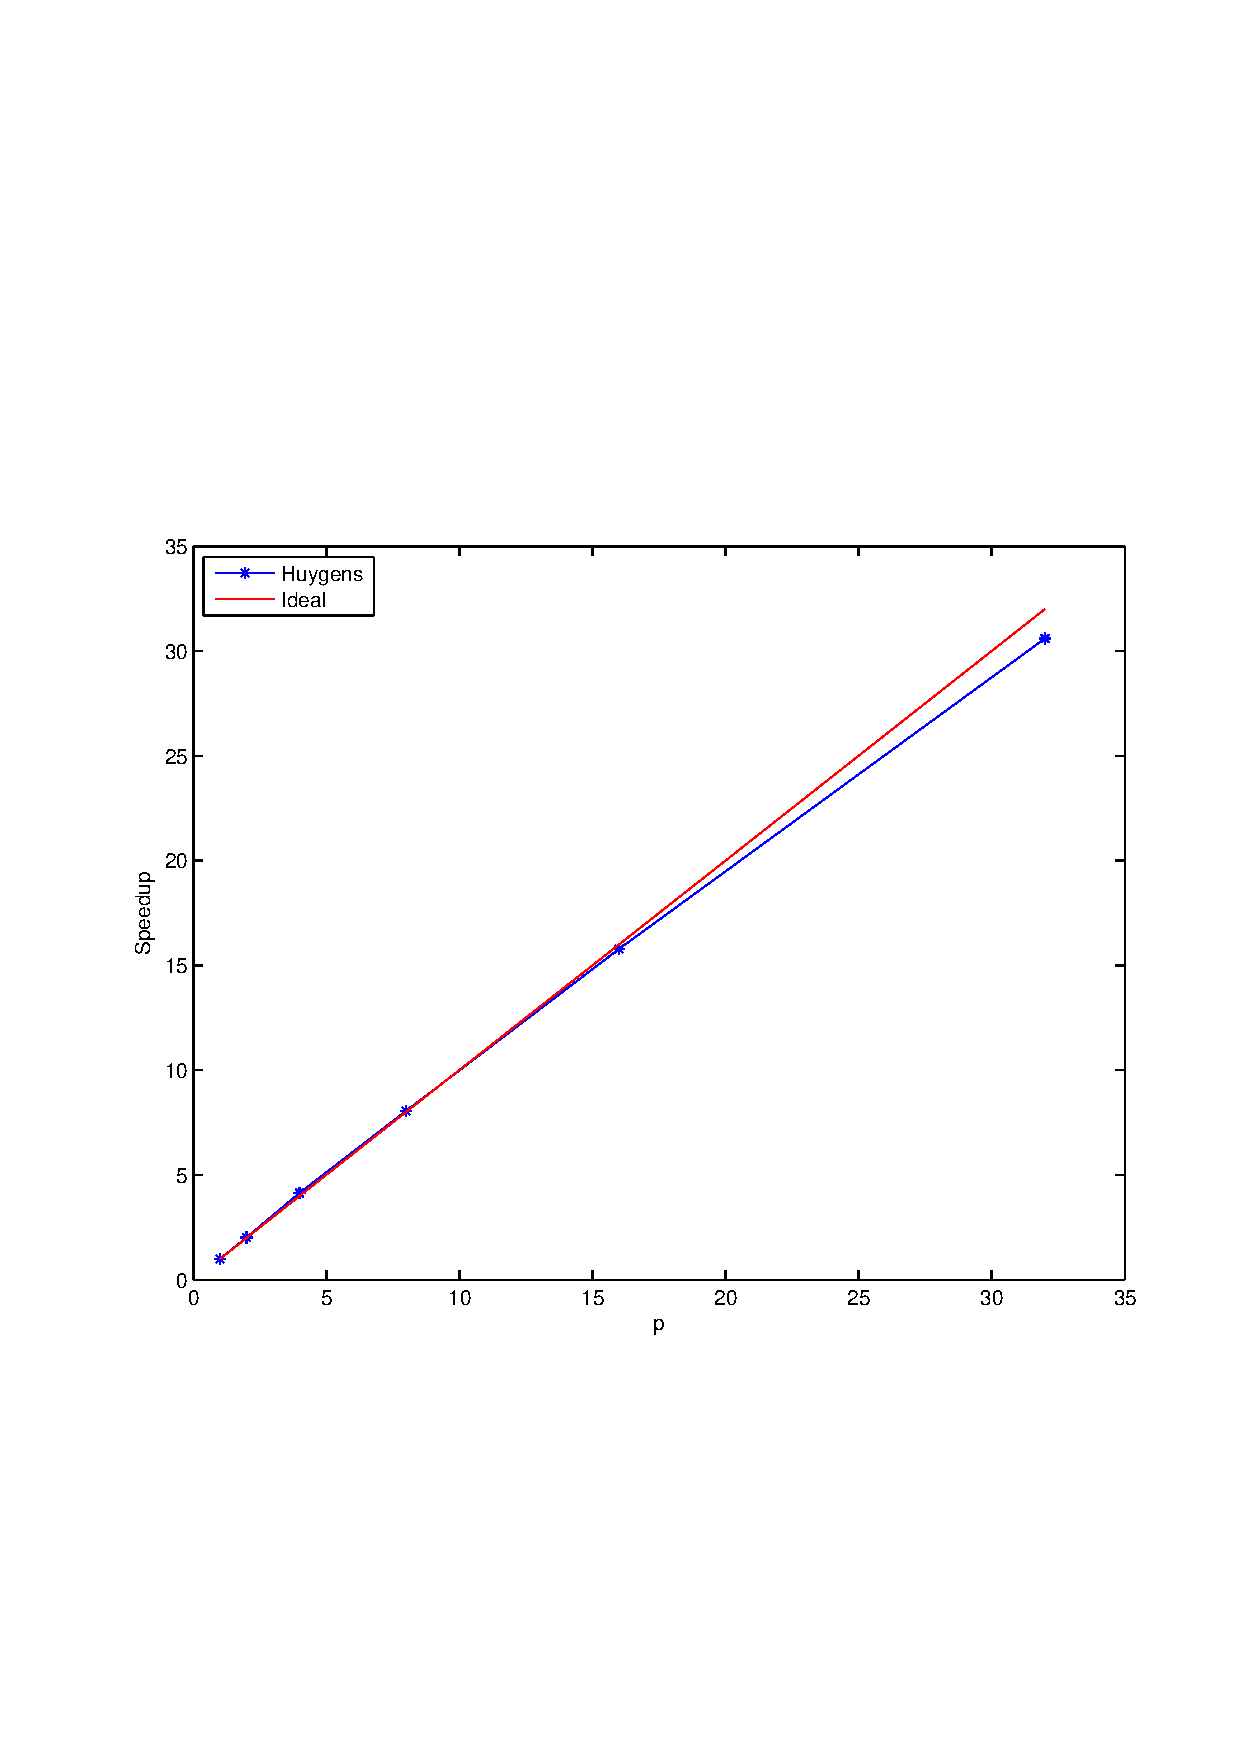
\includegraphics[scale=0.6]{img/sp1e9}
\end{center}
\caption{Speedup plot for Huygens with $n=10^9$} \label{mb:2}
\end{figure}

The results are somewhat surprising, especially for the case $10^8$: from the Figure it is clear that in that case parallelization was well worth the effort! We did not expect the program to improve so much, because parallelization often involves additional costs (communication, synchronization) that slightly worsen the performance. A possible explanation for this is that our initial result (with $p=1$) was particularly bad, which made the other computation look very good. For the case $10^9$ things look much more normal even if it is again a surprisingly good parallelization.

In order to see whether this is the case, we also computed the time with the purely sequential algorithm (described at the beginning of this report) as the $p=1$ case, and we obtained the following speedup plots.

\begin{figure}[H]
\begin{center}
\includegraphics[scale=0.6]{img/sp1e8-2}
\end{center}
\caption{Speedup plot for Huygens with $n=10^8$} \label{mb:2}
\end{figure}

\begin{figure}[H]
\begin{center}
\includegraphics[scale=0.6]{img/sp1e9-2}
\end{center}
\caption{Speedup plot for Huygens with $n=10^9$} \label{mb:2}
\end{figure}

So, it turns out that our sequential algorithm is much faster than the parallel version with $p=1$, and that deeply affects the perspective on the subsequent measurements.		


\subsection{MacBook Air}

In order to gain more insight on the parallelization even on a general purpose computer, we run our parallel sieve also on a MacBook Air.

In the following Tables we outline the results using both MulticoreBSP (denoted by $m$) and BSPonMPI (denoted by $b$) implementations of the BSP model.


\begin{table}[H]
\begin{center}
\begin{tabular}{|C{2.8cm}|r r r|}
\hline
\textbf{n} & p & time $m$  & time $b$ \\
\hline
$10^8$ & 1 &1.150   & 1.3800\\
&2 &0.9921 & 0.9789\\
&4 &0.8375 & 0.8534\\
\hline
$10^9$ &1 &16.277    &17.1801 \\  
&2 &12.4026   &11.8116\\
&4 &11.0896   &11.1477\\
\hline
\end{tabular}
\caption{Time measurements for MulticoreBSP and BSPonMPI for both $10^8$ and $10^9$.} \label{tab:mc_bspmpi}
\end{center}
\end{table}

The speedup plots are shown below:

\begin{figure}[H]
\begin{center}
\includegraphics[scale=0.6]{img/sp1e8m}
\end{center}
\caption{Speedup plot for MacBook Air with $n=10^8$} \label{mb:2}
\end{figure}

\begin{figure}[H]
\begin{center}
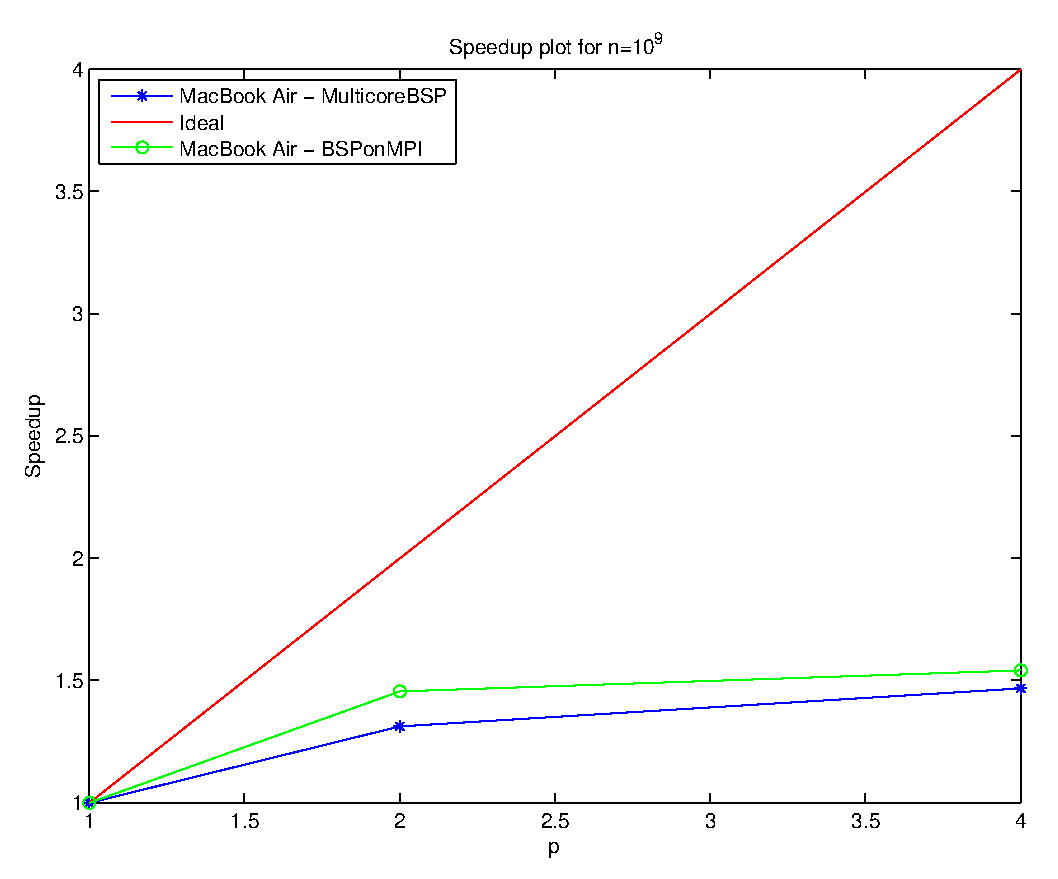
\includegraphics[scale=0.6]{img/sp1e9m}
\end{center}
\caption{Speedup plot for MacBook Air with $n=10^9$} \label{mb:2}
\end{figure}

We can see that BSPonMPI and MulticoreBSP have a very similar behavior, but the latter has the advantage of easier debugging, since we can use the tools normally used for C programming language.

\section{Conclusions}

The whole purpose of this report was to investigate whether the parallelization of the Eratosthenes' Sieve is convenient: from the results we were able to see a significant improvement in the speed of computation of all primes up to the desired $n$, which suggests that it is indeed a very useful approach.

Moreover, we gained more insight on the properties of a supercomputer, being able to look for primes with even 256 processors, and also a new perspective on common laptops, where one might forget that several cores can give a signficant improvement (provided that the program scales well!).


\end{document} 
